% !TeX spellcheck = en_US
\documentclass[en]{../../../eplsummary}
\usepackage{../../../eplunits}

\usepackage{amsmath, amssymb, amsfonts, esvect, mathtools, esdiff}

\usepackage[export]{adjustbox}

\DeclareMathOperator{\supp}{supp}

\hypertitle{Image processing and computer version}{7}{ELEC}{2885}
{Jean-Martin Vlaeminck}
{Christophe De Vleeschouwer and Laurent Jacques}

% Bold for vector notation
\newcommand{\bv}[1]{\mathbf{#1}}
\newcommand{\Hist}{\mathrm{Hist}}
\newcommand{\expand}{\mathrm{Expand}}

\makeatletter
\def\maxwidth#1{\ifdim\Gin@nat@width>#1 #1\else\Gin@nat@width\fi}
\makeatother

\graphicspath{{1-2-image_repr_transforms/}{3-sparsity/}{4-hvs_saliency/}{5-learning/}{6-compressed/}{6-morpho/}{7-segmentation_classification/}{8-comp_photo/}{9-10-tracking/}{11-stereo/}{12-13-compression}}

\part{Introduction and some definitions}
A \emph{two-dimensional digital image} is a matrix of \emph{pixels},
where each pixel has some discrete value in a finite interval
(typically 0 to and including 255), and is defined by
\begin{itemize}
	\item its \emph{resolution}: the amount of pixels in the image,
	and therefore the size of the matrix;
	\item its \emph{depth}: the amount of potential values for each pixel of the image,
	or each element of the matrix;
	\item its \emph{palette} or color system: the way color is encoded
	using the pixels of the matrix.
\end{itemize}

The \emph{resolution} of an image and the \emph{size} of an image
are two different concepts:
two images can have the same resolution (64x64 pixels) but a different size
(e.g., on paper, one is 1 inch by 1 inch when the other is 2 inches by 2 inches),
and two images can have the same size (on paper, 1 inch by 1 inch)
but a different resolution (e.g., 64x64 and 32x32).
The link between the two concepts is the \emph{pixel density}:
the amount of pixels in a direction of a certain length
(e.g., 401 pixels per inch or \SI{401}{ppi}).

Two kinds of resolution:
\begin{itemize}
	\item \emph{resolution of vision (physical image)}:
	the human can look at objects of very different sizes,
	and its resolution can be adapted according to the size of the target object.
	\item \emph{resolution of the digital image}:
	the digital image has a fixed resolution determined by the amount of pixels
\end{itemize}

The \emph{depth} of an image is the amount of values (or \emph{levels}) a pixel can take.
Most of the time, we encode the pixel values using a binary representation
of $b$ bits, and there are $2^b$ levels. The greater the amount of bits $b$ is,
the more (gray) levels a pixel can take.

Example: with $b=8$, we have $256$ levels, ranging from $0$ (black) to $255$ (white).

The human vision is limited to about $6$ to $8$ bits per color,
and therefore maximum $24$ bits for the entire pixel.
Digital images can have a depth much larger than that.

The \emph{palette} gives the way color is represented using the pixels of the image.
The human vision is limited to a palette in the visible spectrum (\num{350} to \SI{700}{nm}).
Digital images can use a wider spectrum (from \SI{0.0001}{nm} to \SI{100}{um}).

\part{Basics of image processing}

\section{Image histogram}

Given an $N$ by $M$ image $I(\bv{x})$, where $I(\bv{x})$ gives the level of pixel $\bv{x}$,
the histogram $\Hist(l)$ is defined by
\begin{equation}
\Hist(l) = \frac{1}{NM} \abs{\{\bv{x} \colon I(\bv{x}) = l\}}.
\label{eq:histogram}
\end{equation}
The histogram gives, for each level $l$,
the amount of pixels of the image that has this level.

\section{Contrast enhancement}
Most of the time, the image uses only a small portion of the available range
of levels. We can therefore improve the contrast by changing the histogram,
and therefore the original values, so that the full range is used.

\subsection{Linear stretch}
\begin{figure}[p]
	\centering
	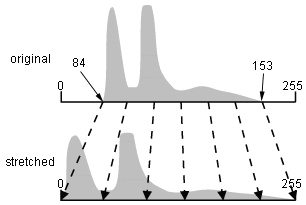
\includegraphics[max width=\linewidth]{linear_stretch}
	\caption{Example of linear stretch}
	\label{fig:1-linear_stretch}
\end{figure}
With $l_\mathrm{min}$ and $l_\mathrm{max}$ being the lower and upper bounds
from the histogram (minimum and maximum brightness values),
we stretch the range $[l_\mathrm{min}, l_\mathrm{max}]$ to fill the full range
and we interpolate the values in-between:
\begin{equation}
l_y = f(l_x) = \frac{255-0}{l_\mathrm{max}-l_\mathrm{min}} (l_x-l_\mathrm{min}).
\end{equation}
See figure~\ref{fig:1-linear_stretch} for an intuitive description.

\subsection{Histogram equalization}
\begin{figure}[p]
	\centering
	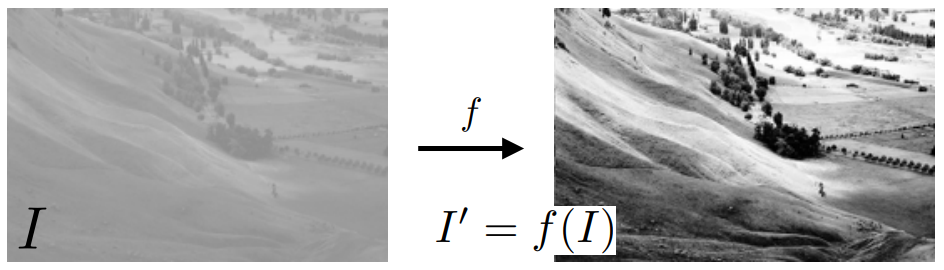
\includegraphics[max width=\linewidth]{hist_equalization_1_1}
	\caption{Example of histogram equalization}
	\label{fig:1-hist_eq}
\end{figure}
Objective: reinstall democracy in pixel levels. This means that levels that are
highly represented in the histogram should be stretched more than levels
that are less represented: this allows a finer scale for highly represented
levels. See figure~\ref{fig:1-hist_eq} for an illustration.

Technically, we want $f\colon [0, L-1] \mapsto [0, L-1]$
such that $\#\{x \colon f(I(x)) \le l\}/N^2 \approx l/L$.
This leads to
\begin{equation}
f(l) = \frac{l-1}{N^2} \abs{\{ x \suchthat I(x) \le l \}}.
\end{equation}

\section{Color spaces}

There exist multiple color spaces: RGB, CMYK, HSI, HSV, YUV\dots
In this course we focus on RGB.
We can view an image as a set of grayscale images, one per color channel.

\section{Frequencies and Fourier analysis}

The Fourier basis functions are
\begin{equation}
\phi_{k, l}(n, m) = \frac{1}{N} \e^{\imagj \frac{2\pi}{N}(nk+ml)}
\end{equation}
with $(n,m)$ being the pixel indices (coordinates in the image),
$(k,l)$ the frequency indices,
$\xi=\frac{2\pi}{N}\binom{k}{l}$ the frequency vector,
$\norm{\xi}$ the frequency amplitude,
$\angle(\xi)$ the frequency angle.

The discrete Fourier transform (DFT) for a 2-D image is
\begin{equation}
F(k, l) = \frac{1}{N} \sum_{n=0}^{N-1} \sum_{m=0}^{N-1} f(n, m) \e^{-\imagj (2 \pi / N) (nk + ml)}
\end{equation}
and the inverse transform is
\begin{equation}
f(n, m) = \frac{1}{N} \sum_{k=0}^{N-1} \sum{l=0}^{N-1} F(k, l) \e^{+\imagj (2 \pi / N) (nk + ml)}.
\end{equation}
The Fourier transform can be interpreted as computing the projection of $f$ on or scalar product of $f$ with $\phi_{k,l}^*$.

From this definition, we define the DC value or image mean as $F(0,0)$,
and the AC values as the other values.

Usually, the result of the Fourier transform is full of complex numbers,
and we need both the amplitude and the phase of $F(k,l)$ to recover $f$.

% I stopped at slide 30/85
% TODO speak about the FFT, the properties of masking, log-scale graphs

% Restart at 61
\section{Multi-scale transformations}

The Fourier transform has the limit that it transforms the signal
in a frequency domain. This means that the time component is completely
transformed and mixed into different coefficients of the transform.
We would like a representation in a time-frequency domain, similar to musical
scores, that tells in a local neighborhood of the image what frequencies
are present and what the structure of the signal is.

\subsection{Laplacian pyramid}

As a first example (others will come later), we present the Laplacian pyramid.
This representation performs an analysis of the image details at different scales.

We define
\[ L_k = g_k - g_{k+1} = g_k - g_k \ast h \]
as the map of details of the image at level $i$ (it is similar to the result
of applying a Laplacian operator to the image).
$h$ is usually a Gaussian filter $h(n,m) = c \exp(-\frac{1}{2}(n^2+m^2))$.
However, we don't define $g_{i+1}$ as $g_i \ast h$, bu rather as
a downsampled version of $g_i \ast h$, such that we can keep our filter $h$
but work at a scale that is larger. We need an operation, $\expand$, to go
from this downsampled version to a version of similar size than $g_i$,
to define
\begin{equation}
L_k = g_{k-1} - g_k' = g_{k-1} - \expand(g_k).
\end{equation}
In our context of a $\expand$ can be defined
Starting from $k=1$, we can construct every $L_k$, up to a given level $K$
(e.g. $K=5$) where we need to store both $L_K$ and $g_K$.
The Laplacian transform is then each $L_1,\dots,L_K$, and $g_K$, and we can
process each level independently before reassembling the image with the relation
\begin{equation}
g_{k-1} = \expand(g_{k}) + L_{k}
\end{equation}
starting from $k=K$ down to $0$.

For a subsampling of $\frac{1}{2}$, the output of this transformation has about
$\frac{4}{3}$ the number of pixels than the original image. This feels useless,
but actually we have unfolded the image by scale and resolution of details.

Additional details: upsampling can be achieved either by interpolating
$g_k'$ to obtain $g_k$ (any interpolation will work because it will be taken
into account inside the corresponding $L_k$ at the generation step)
or by moving it in the Fourier domain, zero-pad around this domain (to obtain
a $4$ times larger domain), then converting back to the pixel domain.
Likewise, any reasonable function $h$ and any reasonable  downsampling
can be used, and this will be taken into account in $L_k$. However, it is
important that these three functions are common to the forward and
to the backward procedures, less we won't be able to reconstruct the image.

\section{Wavelet transform}

Note: this section is here because it fits more with the previous subjects
of transformations from one base to another, even though its most significant
applications are covered in the next section.

\subsection{General idea}

The general idea of wavelet transforms is to look for a way to describe
discretely and imperfectly a continuous-time signal such that temporal locality
is exploited to yield a more straightforward interpretation than the Fourier
transform, that often produces a complete but messy set of coefficients.

We start by building a piecewise constant approximation to the signal $f(t)$.
For this, given a resolution $\Delta t$, we compute the mean in each interval
$[k\Delta t, (k+1)\Delta t]$. This mean is calculated by evaluating
the correlation of $f$ with a \emph{scaling function}
$\phi_k(t) = \frac{1}{\sqrt{\Delta t}} \phi(\frac{t}{\Delta t} - k)$,
where $\phi(t) = 1$ if $0 < t < 1$ and $0$ otherwise:
\[ c_k = \langle f, \phi_k \rangle = \frac{1}{\sqrt{\Delta t}} \int_{k\Delta t}^{(k+1)\Delta t} f(t) \dif{t}. \]
From this,
\[ f_\mathrm{app}(t) = \sum_k c_k \phi_k(t) = \sum_k \langle f, \phi_k \rangle \phi_k(t). \]
We can say that $f$ was projected on an \emph{approximation space}
$\mathcal{V}(\Delta t)$ containing all the functions that can be approximated
using constant piecewise functions of scale $\Delta t$, and which has
an orthonormal basis (ONB) given by $\phi_k$ for $k\in \N$.

We can then do a finer approximation by using a scale of $\Delta t/2$.
Then, the difference between the two approximations happens to contain
the details of the signal at this scale.

Let's formalize it a bit: we assume $\Delta t=1$, so that we have
\[ \mathcal{V}_j = \{ \phi_{j,k}(t) = 2^{j/2} \phi(2^j t - k) \forall k \in \Z \} \]
and $f_j(t) = \mathcal{P}_{\mathcal{V}_j} f$. With increasing $j$, $f_j$
are an increasingly finer approximations of $f$. $j=0$ often corresponds
to $\Delta t$ being the full length of the signal. We have that $\forall i \le j,
f_i = \mathbb{P}_{\mathcal{V}_i} f_j$.

Then, $d_j(t) = f_{j+1}(t)-f_j(t) \in \mathcal{W}_j$ can be considered, and are
the details of the signal. They all belong to a space, $\mathcal{W}_j$, such that
$\mathcal{V}_{j+1} = \mathcal{V}_j \oplus \mathcal{W}_j$; $\mathcal{W}_j$ is
orthogonal to space $\mathcal{V}_j$ and together they form $\mathcal{V}_{j+1}$.
We can also write $f_{j+1}(t) = d_j(t) + f_j(t)$ to notice that we are applying
a multiscale transformation alike the Laplacian pyramid.

The space $\mathcal{W}_j$ has an ONB given by
\[ \{\psi_{j, k}(t)=2^{j/2} \psi(2^{j} t - k)\}, \] % FIXME there is an error in the slides
where $\psi(t) = -1$ if $0 < t < \frac{1}{2}$, $1$ if $\frac{1}{2} < t < 1$, and $0$ otherwise;
this is what we call a \emph{wavelet}. We can also write
\begin{equation}
d_j(t) = \sum_k \langle f, \psi_{j,k} \rangle \psi_{j,k}(t) = \mathcal{P}_{\mathcal{W}_j}(f_{j+1}).
\end{equation}

\subsection{Multiresolution analysis (MRA)}

For this, we assume that $f$ is sampled at highest resolution $J$, that is
$f(t)=f_J(t)=\mathcal{P}_{\mathcal{V}_j}f_\mathrm{cont}$.
From $f_j$, we can calculate
\[ f_{j-1} = \mathcal{P}_{\mathcal{V}_{j-1}} f_j \]
and
\[ d_{j-1} = \mathcal{P}_{\mathcal{W}_{j-1}} f_j. \]
We finally only keep the $d_j$ signals for $0 \le j \le J-1$ as well
as the function corresponding to the mean $f_0$ to have our
\emph{wavelet transform} coefficients, and the process just described
is exactly the basic computation of the $N$ wavelet coefficients.

The inverse transform is then
\[
f_J(t) = (\dots((f_0+d_0)+d_1)\dots+d_{J-1})
  = \sum_{j=0}^{J-1} \sum_k \langle f_J, \psi_{j,k} \rangle \psi_{j,k}(t)
  + \sum_k \langle f_J, \phi_{0,k} \rangle \phi_{0,k}(t)
\]

\subsection{Fast Wavelet Transform (FWT)}

As with FFT for the DFT, we have a FWT for the DWT: the idea is that
\begin{alignat*}
\phi(t) &= \frac{1}{\sqrt{2}} & (\sqrt{2} \phi(2t)) &+ \frac{1}{\sqrt{2}} (\sqrt{2} \phi(2t-1)) \\
\psi(t) &= -\frac{1}{\sqrt{2}} & (\sqrt{2} \psi(2t)) &+ \frac{1}{\sqrt{2}} (\sqrt{2} \psi(2t-1))
\end{alignat*}
so we can compute the coefficients at level $j$ from the coefficients at level $j+1$:
% TODO put the graph of the circuit for computing this (slide 44)

\subsection{Wavelet types}

There are different types of wavelets:
Haar wavelets (those we studied in the course),
Daubechies wavelets (commonly used in algorithms, like JPEG2000),\dots

\subsection{Extension to images}

We apply a principle of separability: approximations are formed by computing
the correlation of $f$ with $\phi(x)\phi(y)$ (for mean value),
$\phi(x)\psi(y)$ (for horizontal features or vertical details),
$\psi(x)\phi(y)$ (for vertical features or horizontal details),
and $\psi(x)\psi(y)$ (for bi-diagonal features).

We then execute the algorithm by first applying it vertically, to yield
two horizontal rectangles, and then applying it horizontally, to yield
four squares.
The bottom right one is usually $d_{J-1}^D$ (bi-diagonal component, HH),
the bottom left is $d_{J-1}^V$ (vertical features are apparent, LH),
the top right is $d_{J-1}^H$ (horizontal features, HL),
and the top left is the mean $a_{J-1}$ (LL), on which we can reapply
our algorithm to finally yield a sufficiently small $a_0$.

\part{Redundant bases and sparsity: principles, properties and applications}

\section{Sparsity basis}

\begin{myhyp}
	Any signal can be decomposed in a \emph{sparsity basis} $\Psi$
	with few non-zero elements $\alpha$:
	\[ f(m) = \sum_{k=1}^{d} \alpha_k \psi_k(m), \quad \Psi = \{ \psi_j\colon 1 \le j \le d \} \]
	and $\supp(\alpha)$ (the \emph{support} of $\alpha$, or the number
	of nonzero elements) is small compared to the size of $\Psi$.
\end{myhyp}

$\Psi$ can be anything: an ONB (including Fourier basis, wavelets basis),
a frame (ridgelets, curvelets), or can be redundant.

\section{Redundant system}

A system (more precisely, a basis) $\Psi$ is redundant if there exist signals
that can be represented by two different ways using $\Psi$, and that every signal
can be represented in $\Psi$.

If $N$ is the length of the signal of interest, then
$\Psi = \{ \psi_k \in \R^N \colon 1 \le j \le d \}$ with $d >> N$.
The dictionary hence contains more atoms $\psi_k$ than required,
and $\Psi \Psi^\Tr \neq I_N$: this is not an othonormal basis, and we need
new algorithms to compute this.

An example of redundant system is the combination of the Fourier basis functions
with the canonical basis (Dirac deltas at each point): this car represent
sparsely (i.e., with few non-zero components) a sine with two brusque deltas
(4 components in total, instead of $N$).

Another example of redundant dictionary starts from a mother function $\psi(t)$,
and applies different transformations to it:
translation $T_b\psi(t) = \psi(t-b)$,
dilation $D_a\psi(t) = \frac{1}{\sqrt{a}} \psi\left(\frac{t}{a}\right)$,
and modulation $M_\omega \psi(t) = \psi(t) \exp(2\pi \imag \omega t)$.
this is to be compared with the short-time Fourier transform
(used for spectrogram; see figure~\ref{fig:3-redundant_ex1} for an example),
which combine translation and modulation, and with the wavelet transform,
which combines translation and scaling.

\section{Sparse recovery problem}

Given a signal $x \in \R^N$ and a dictionary of atoms $\Psi \in \R^{N \times d}$
with $d >> N$, we want to find $\alpha \in \R^d$ such that $x=\Psi \alpha$.

This problem has an infinite number of solutions as the dictionary is redundant
(if it had been orthonormal, there would be only one solution);
we want to find the sparsest solution, the solution that minimizes
$\supp(\alpha)$.

However, this problem cannot be solved with our existing technique
of correlations, as $\Psi \Psi^\Tr \neq I_N$; we need new algorithms to solve
\[ \alpha = \arg \min \norm{\alpha'}_0 \text{ such that } x = \Psi \alpha'. \]

\section{Algorithms for the sparse recovery problem}

Let's first point out that the sparse recovery problem is actually NP-hard.

\subsection{Basis pursuit}

Proposed by Chen, Donoho ans Saunders in 1998, after MP and OMP.

The idea is to relax the constraint of sparsity from the $l_0$ norm
to the $l_1$ norm (sum of absolute values) to obtain
\begin{equation}
\alpha = \arg \min \norm{\alpha'}_1 \text{ such that } x = \Psi \alpha'.
\end{equation}

This is justified by the fact that $x=\Psi \alpha$ defines a $d$-dimensional line
and we want to find its (ideally unique) intersection with the smallest
$l_0$ ball (which is just the set of axes limited to some value).
We can replace the $l_0$ ball with the $l_1$ ball (actually a rhombus),
as most intersections of a random line with the smallest rhombus possible
will happen on the axes. See figure~\ref{fig:3-bp_norms} for an intuition.

\begin{figure}[p]
	\centering
	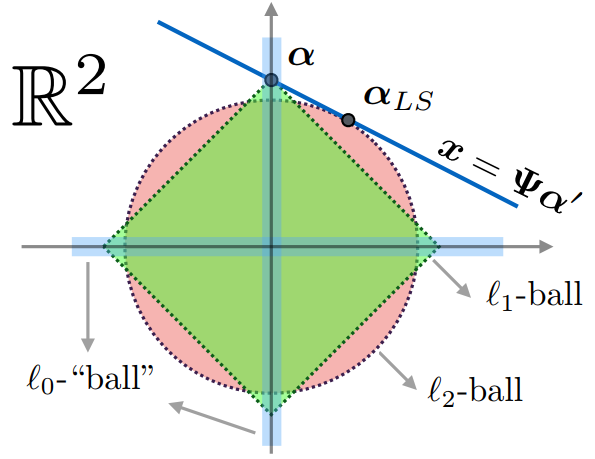
\includegraphics[width=\maxwidth{\linewidth}]{basis_pursuit_norms}
	\caption{A comparison of the smallest $l_0$, $l_1$ and $l_2$ balls that
	intersect with the line $x=\Psi \alpha$}
	\label{fig:3-bp_norms}
\end{figure}

A big advantage of this method is that the resulting problem becomes
a linear program (a set of linear inequalities as constraints),
and there exists a lot of different and efficient methods to solve such problems.

\subsection{Matching pursuit}

\subsection{Orthogonal matching pursuit}

\subsection{Iterative hard thresholding}

\begin{figure}[p]
	\centering
	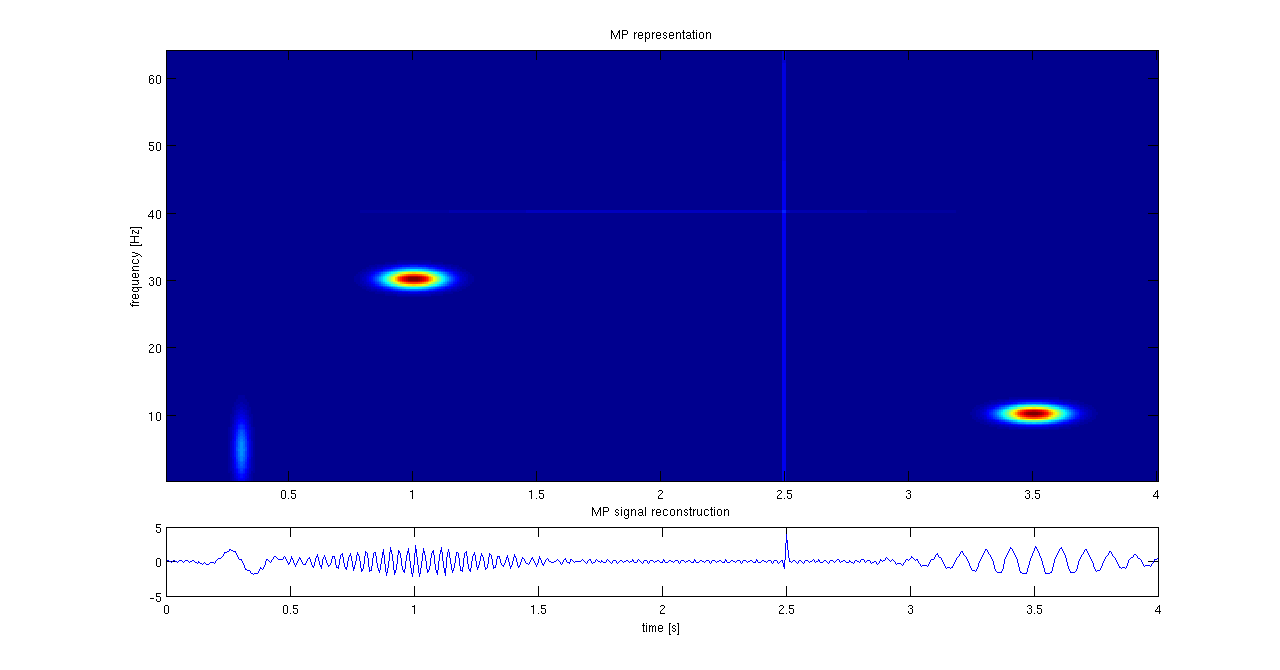
\includegraphics[width=\maxwidth{\linewidth}]{Matching_pursuit.png} % Source: Wikipedia, "Matching pursuit"
	\caption{1-D example of the short-term Fourier transform of a 1-D signal,
	using matching pursuit.}
	\label{fig:3-redundant_ex1}
\end{figure}

\part{Mathematical morphology and relatives}

\begin{mydef}
	Mathematical morphology is a theory and technique that applies concepts from set theory,
	lattice theory\footnote{A lattice is a structure consisting of
		a partially ordered set\footnote{A set where every pair of elements \emph{may} be compared}
		where every two elements have a unique infimum or greatest lower bound or meet
		and a unique supremum or least upper bound or join.
		An example is the natural numbers, ordered by divisibility,
		with the infimum being the GCD and the supremum being the LCM.
	}, and topology, to the analysis and processing of geometrical structures.
\end{mydef}
In practice, we define a set of \emph{morphological operators} (typically set operators)
between an image and a \emph{structuring element}, that will transform these images.

A \emph{structuring element} is a simple, generic shape used to probe the image
in order to draw conclusions on whether the shape fits in the image.
Examples are $n$-by-$n$ matrices of ones, or crosses of ones, or disks of ones.
The points inside these basic shapes can be either $1$ or ``don't care's''.
We can also extend the definition to include sophisticated shapes which can contain $0$.

For \emph{binary morphology}, we consider an image as being just a set of points
belonging to the bright part of the image: there is only two levels in the quantized intensity.
The morphological operators are only set operators and combinations of them.

For \emph{grayscale morphology}, we consider the regular definition of an image,
and the morphological operators can be interpreted as convolutions in a tropical geometry.

\begin{mynota}
	\begin{itemize}
		\item $X$ defines a binary image as a set of pixel coordinates.
		\item $K$ defines a set of pixel coordinates for the structuring element.
		\item $K_x$ is the structuring element translated in $x$.
		\item $K^s$ is the symmetrization of the structuring element: $\{ -x \suchthat x \in K\}$
	\end{itemize}
\end{mynota}

\section{Basic operators}

\subsection{Dilation}

Dilation enlarges the boundaries of regions of foreground, white pixels on a binary image.

\begin{equation}
X \oplus K = \{ x \suchthat K_x \cap X \neq \emptyset \}
\end{equation}

\paragraph{Properties}
\begin{itemize}
	\item Commutativity: $A \oplus B = B \oplus A$.
	\item Associativity: $A \oplus (B \oplus C) = (A \oplus B) \oplus C$.
	\item Extensivity: if $0 \in B$, then $A \subseteq A \oplus B$.
	\item Dilation is increasing: $A \subseteq B \implies A \oplus D \subseteq B \oplus D$.
	\item When dilating by a disk-shaped structuring element,
	convex boundaries will become rounded (i.e., outside corners become rounded),
	and concave boundaries are preserved in shape but are translated towards
	the empty inside space (i.e., inside corners are left as is).
\end{itemize}

Binary dilation can be used for edge detection: $(X \oplus K) \setminus X$ leaves the edges.

Binary dilation can be used for region filling:
with a structuring element $K$ and the complementary of the image $A^c$
\footnote{This image contains the boundary of the region of interest.}
starting from a unique point $X^{(0)}$ inside a region of interest,
compute $X^{(k)} = (X^{(k-1)} \oplus K) \cap A^c$ iteratively.
When the process converges, $X^{(k)} \cup A$ defines the filled region.

\paragraph{Grayscale dilation}
The grayscale dilation, for a regular image $f$ and a structuring element $b$
defined over a region $E$, is
\begin{equation}
(f \oplus b)(x) = \sup_{y \in E} (f(y) + b(x - y))
\end{equation}

This equation can be interpreted as a convolution in tropical geometry:
\begin{mydef}
	Tropical geometry, or max-plus algebra\footnote{A min-plus algrebra is also
		a tropical geometry, but is not used in this course},
	is a version of geometric algebra using a \emph{tropical semiring} instead of a field.
	A tropical semiring is a semiring of extended real numbers
	$\R \cup \{+\infty, -\infty\}$ with the operations of maximum and addition
	replacing the usual addition and multiplication operations.
\end{mydef}

The convolution $(f \star g)(x) = \int f(t) \times g(x-t) \dif{x}$ is thus transformed
into $(f \oplus g)(x) = \sup f(t) + g(x-t)$.

Grayscale dilation has the effect of brightening the image, as bright regions
surrounded by dark regions grow in size, and dark regions surrounded by
bright regions shrink in size.

Grayscale dilation can also remove pepper noise: dark points in the image.

\subsection{Erosion}

Erosion is the dual of dilation: it erodes away the boundaries of regions
of foreground, white pixels.

\begin{equation}
X \ominus K = \{ x \suchthat K_x \subseteq X \}
\end{equation}

\paragraph{Properties}
\begin{itemize}
	\item Erosion is \strong{not} commutative nor associative.
	\item Extensivity: if $0 \in B$, then $A \ominus B \subseteq A$.
	\item Dilation is increasing, but in the other direction:
	$A \subseteq C \implies (A \ominus B \subseteq C \ominus B)$
	and $B \supseteq C \implies (A \ominus B) \subseteq A \ominus C$.
	\item Chain rule: $A \ominus (B \oplus C) = (A \ominus B) \ominus C$.
	\item Translation invariance: $A_x \ominus B = (A \ominus B)_x$
	and $A \ominus B_x = (A \ominus B)_{-x}$.
	\item Linearity: $(A \cap B) \ominus C = (A \ominus C) \cap (B \ominus C)$.
	\item Containment: $A \cup B) \ominus C \supseteq (A \ominus C) \cup (B \ominus C)$.
	\item Decomposition of structuring elemnts:
	$A \ominus (B \cup C) = (A \ominus B) \cap (A \ominus C)$.
	\item When eroding by a disk-shaped structuring element,
	convex boundaries will be preserved, and concave boundaries will be rounded.
\end{itemize}

\paragraph{Grayscale erosion}
Using the same notation as for dilation,
\begin{equation}
(f \ominus g)(x) = \inf_{y \in E} (f(y) - b(x-y))
\end{equation}
which can be considered as a convolution in a min-minus algebra (still a tropical geometry).

Grayscale erosion has the effect of darkening the image, as dark regions
surrounded by bright regions grow in size, and bright regions surrounded by dark
regions shrink in size.

Example applications: separating objects that are initially touching each other,
remove salt noise (white points on the image).

\subsection{Opening}

Opening is defined as an erosion followed by a dilation:
\begin{equation}
X \circ K = (X \ominus K) \oplus K
\end{equation}

The effect of binary opening is that regions matching the structuring shape are
preserved, so that the resulting image could have been drawn from
a structuring-element-shaped brush.
Equivalently, the new foreground region will be such that the structuring
element fits inside it.
Similarly to erosion, the resulting image is included within the original image:
it removes some of the foreground pixels.
An important effect of opening is idempotence:
$(X \circ K) \circ K = X \circ K$, meaning that subsequent applications of opening
don't change the image.

\paragraph{Examples}
In figure~\ref{fig:6-opening-ex1}, with a disk-shaped structuring element
of the same size as the disks, we can see that the lines were removed from
the image while the circles have been mostly unaffected.
\begin{figure}
	\centering
	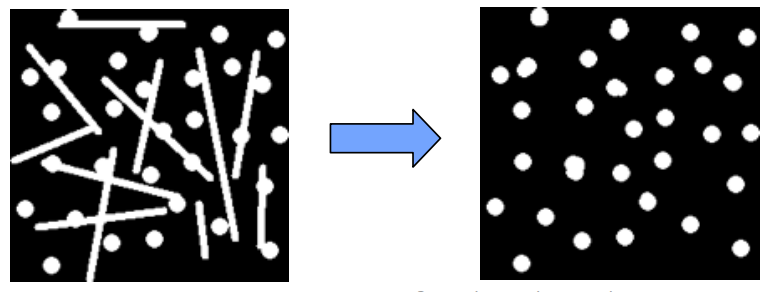
\includegraphics[max width=\linewidth]{opening_example1.png}
	\caption{Example 1 of opening}
	\label{fig:6-opening-ex1}
\end{figure}

In figure~\ref{fig:6-opening-ex2}, with a 5-by-5-square-shaped structuring element,
we can see that the bright features smaller than the shape have been reduced
in intensity.
\begin{figure}
	\centering
	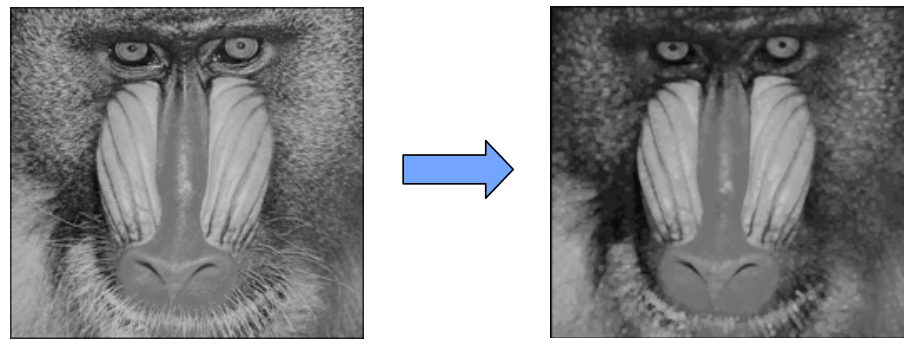
\includegraphics[max width=\linewidth]{opening_example2.png}
	\caption{Example 2 of opening}
	\label{fig:6-opening-ex2}
\end{figure}

In figure~\ref{fig:6-opening-ex3}, opening removes the salt noise and doesn't degrade
the image as much as a regular erosion.
However, opening can't remove pepper noise: it will even increase the noise!
\begin{figure}
	\centering
	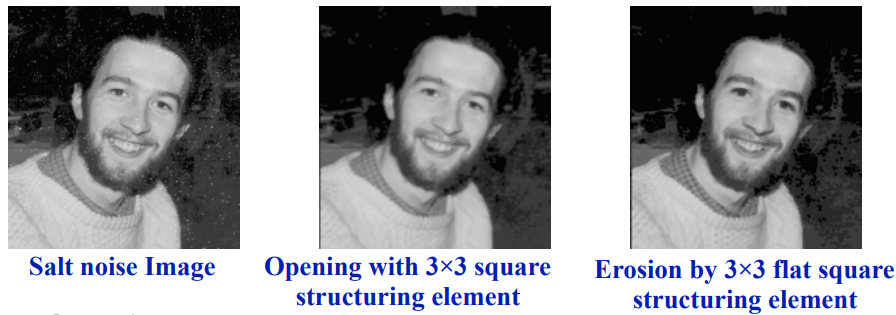
\includegraphics[max width=\linewidth]{opening_example3.png}
	\caption{Example 3 of opening}
	\label{fig:6-opening-ex3}
\end{figure}

\subsection{Closing}

Closing is defined as a dilation followed by an erosion:
\begin{equation}
X \bullet K = (X \oplus K) \ominus K
\end{equation}
Similarly to dilation, the resulting image contains the original image:
it grows the image boundaries. We also have idempotence for closing.
The new background regions will be such that the structuring element can cover
any point in the background without covering a point from the new foreground region.

\paragraph{Properties of opening and closing}
\begin{itemize}
	\item Translation invariance: $A \circ B_x = A \circ B$
	and $A \bullet B_x = A \bullet B$.
	\item Antiextensivity of opening: $A \circ B \subseteq A$.
	\item Extensivity of closing: $A \subseteq A \bullet B$.
	\item Duality: $(A \bullet B)^c = A^c \circ B^s$.
\end{itemize}

\paragraph{Examples}
In figure~\ref{fig:6-closing-ex1}, we can remove the small holes by closing.
\begin{figure}
	\centering
	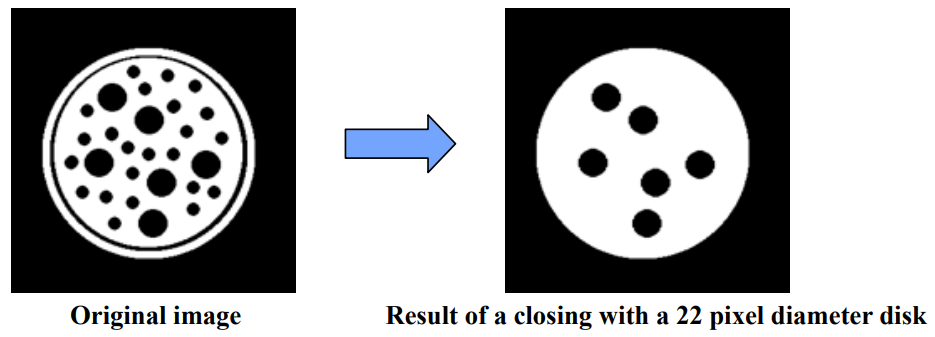
\includegraphics[width=\maxwidth{\linewidth}]{closing_example_1.png}
	\caption{First example of closing}
	\label{fig:6-closing-ex1}
\end{figure}

In figure~\ref{fig:6-closing-ex2}, we can reduce the complexity of the skeleton
by closing the thresholded image first
\begin{figure}
	\centering
	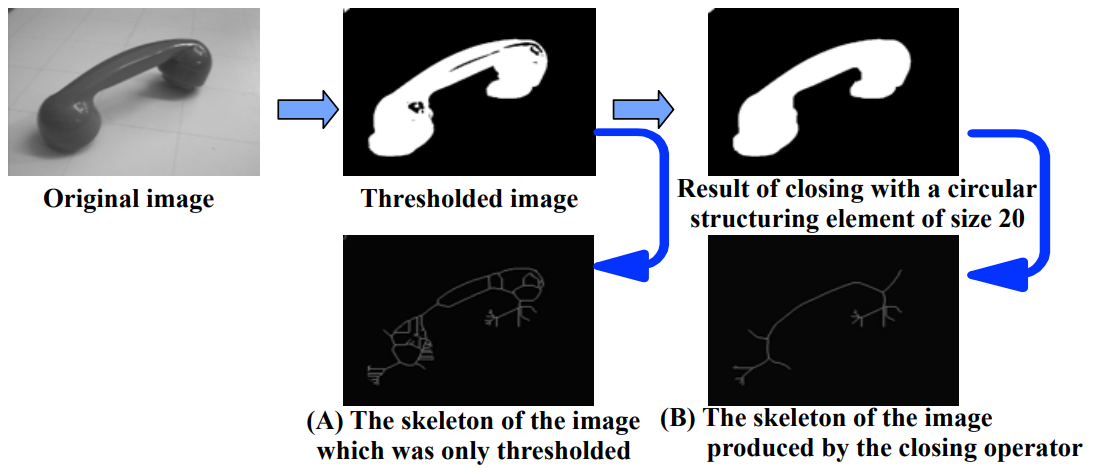
\includegraphics[width=\maxwidth{\linewidth}]{closing_example2.png}
	\caption{Second example of closing}
	\label{fig:6-closing-ex2}
\end{figure}

And of course, closing can remove pepper noise, but fails to remove salt noise.

\section{Morphological filtering}

We can use the previous algorithms to identify various geometrical structures
and properties of the image, by varying the shape and the size
of the structuring elements.

\section{Morphological pyramid}

Idea: replace convolution (in the subsampling stage) by morphological dilation
in the Gaussian/Laplacian pyramids.
The equations and the construction of the pyramid is otherwise similar to that of a regular Laplacian pyramid.

\section{Some more advanced concepts}

Not seen in 2018-2019.

\subsection{Hit-and-miss transform}

Not seen in 2018-2019.

\subsection{Thinning}

Not seen in 2018-2019.

\subsection{Thickening}

Not seen in 2018-2019.

\subsection{Skeletonization and Medial Axis Transform}

Not seen in 2018-2019.

\part{Image segmentation}

\section{Edge detectors}

\begin{mydef}
	In 1-D, an edge is a point where the first derivative of the ``intensity''
	is maximum. And thus, where the second derivative is zero.
\end{mydef}
\begin{mydef}
	In 2-D, an edge is made of points where the first directional derivative
	of the ``intensity'' is maximum along the direction of its gradient.
\end{mydef}

Given a point $\vv{x}=(x, y)^\Tr$, the gradient is
\[\vv{\nabla} I(\vv{x}) = \left(\diffp{}{x}I(\vv{x}), \diffp{}{y}I(\vv{x})\right)^\Tr\],
the directional derivative in unitary direction $\vv{u}=(u_x, u_y)^\Tr$ is
\[\diff{I}{x}(\vv{x}) = u_x \diffp{I}{x}(\vv{x}) + u_y \diffp{I}{y}(\vv{y})\]

If we define $\vv{u}=\frac{\vv{\nabla}I(\vv{x})}{\norm{\vv{\nabla}I(\vv{x})}}$,
$J(\lambda) = I(\vv{x}+\lambda \vv{u})$, then $\vv{x}$ is part of an edge
if $J'(\lambda)=\vv{\nabla}I(\vv{x}+\lambda \vv{u})\cdot \vv{u}$
is locally maximum in $\lambda=0$. In other words, if
\[ \vv{u}^\Tr \begin{pmatrix} \diffp{I}{{x^2}} & \diffp{I}{{x}{y}} \\ \diffp{I}{{x}{y}} & \diffp{I}{{y^2}} \end{pmatrix} \vv{u} = 0 \].

However, this technique can't be used, as the image $I$ is a discontinuous function.

General idea: smooth the image before applying the previous method.
We define $g_\sigma$ as a Gaussian of scale $\sigma$, and we define
$I_\sigma = I \ast g_\sigma$, and thus
\[ \vv{\nabla}I_\sigma(\vv{x}) = I \ast \vv{\nabla} g_\sigma \].
This gives the edges available at scale $\sigma$.

\subsection{Canny-Lindeberg detector}

The Canny-Lindeberg edge detector is a direct application of this principle,
with the details worked out.
There is a trade-off between the edge accuracy and the noise resistance:
at finer scales $\sigma$, the edges are more accurately detected and tracked,
but there are a lot of noisy edges due to the inherent noise;
at large scale, there are less noisy edges and less noise, but the edges are
inaccurate and often disconnected from each other.

Lindeberg designed a method for automatically choosing the best value for the scale.

\subsection{Watershed method}

This is a pixel-based segmentation. The basic idea is that we have
a rising ``water level'', that fills the various parts of the image under
the image intensity surface, and each time two separate regions are merged
together at a junction due to the rising water, we record the junction as part
of an edge, that will end when another regions merges with the two first.

This algorithm has the default of creating a lot of regions
(due to irregularities within a single region), and we need to merge them.
We can build a Region Adjacency Graph, and merge the regions based
on similar size, similar mean color, the boundary length,
\dots\footnote{Visually, the results are still pretty bad.}

\section{Feature-based segmentation}

A \emph{feature vector} is associated to each pixel and contains various types
of information about this pixel. Examples include:
\begin{itemize}
	\item colors (in YUV, RGB, HSV, HSL systems);
	\item spatial gradients (2 components);
	\item velocity of the pixel on the image (2 components; only for video);
	\item texture content around a pixel (stationarity, variance).
\end{itemize}
These features can be computed by image processing.

Using these feature vectors and working in the feature space, we can
segment our image, i.e., separate the image into regions, by assigning
each pixel to a semantic descriptor as well as a confidence measure.

Hypothesis: coherence and redundancy among features in a region (pixels
in a region share similar feature vectors).

\subsection{Clustering}

Build clusters of similar feature vectors and assign them to the same region.

Clusters are defined by a set of centroids, $\mathcal{C}$, with one centroid
per cluster. And we want to find
\[ \mathcal{C}^\mathrm{opt} = \arg \min_{\mathcal{C}} (\phi_\mathcal{C} = \sum_{x \in \mathcal{X}} \min_{c \in \mathcal{C}} \norm{x-c}^2) \]
which is a NP-hard problem. We must thus find approximate methods.
Examples are $K$-Means (or Lloyd-Max), with various different initializations
like $K$-Means++.

$K$-Means++ algorithm:
\begin{enumerate}
	\item set $\mathcal{C}^0 = \{c_1\} \in \mathcal{X}$ with $c_1$ picked
	uniformly at random in $\mathcal{X}$ (initially one centroid).
	\item for $k=2$ to $K$ do:
	\begin{enumerate}
		\item Compute the distances $D(u, A) = \min_{a \in A} \norm{u-a}$,
		the sum of the squared distances $S=\sum_{x \in \mathcal{X}} D(x, \mathcal{C}^0)^2$,
		and the probability mass function $p(x) = \frac{1}{S} D(x, \mathcal{C}^0)^2$.
		\item Pick $c_k$ at random in $\mathcal{X}$ according to $p$.
		\item $\mathcal{C}^0 \leftarrow \mathcal{C}^0 \cup \{c_k\}$.
	\end{enumerate}
	\item Run $K$-Means with initial cluster $\mathcal{C}^0$.
	\item Repeat steps 1 to 3 several times and select the best $\mathcal{C}^0$.
\end{enumerate}
This algorithm can guarantee that
\[ E_{\mathcal{C}^0} \phi(\mathcal{C}_{\text{K-Means++}}) \le 8 (\ln K + 2) \phi(\mathcal{C}^\mathrm{opt}) \]

The thematic of clusters is reviewed in more details in the course of Machine Learning, LELEC2870.

\subsection{Clustering in other geometries: spectral clustering}

If the geometry of the feature space is not appropriately specified by
a cluster of convex sets (e.g., one set is inside another set that is annular,
with small inside-cluster distances and large inter-cluster distances),
we have to do \emph{spectral clustering}.

\begin{mydef}
\emph{Spectral clustering}: Define a graph from data in order to learn
intrinsic data geometry and cluster thanks to the frequencies of the graph.
\end{mydef}

\paragraph{Reminders about graphs}
We can define a graph $\mathcal{G} = (V, E, W)$ by
its vertices $V=\{v_i\}_{i=1}^N$,
its edges $E=\{(v_i, v_j)\suchthat v_i \sim v_j\} \subset V \times V$
and its weights $W=\{w_{ij}\suchthat w_{ij} \neq 0 \text{ if } (v_i, v_j) \in E\}$.

An undirected graph has the additional properties that
$(v_i,v_j) \in E \Leftrightarrow (v_j, v_i) \in E$ and $w_{ij} = w_{ji}$.

We can define graphs using the \emph{adjacency matrix} containing $w_{ij}$.

\paragraph{Laplacian of the graph and connected components}
We first define the \emph{graph Laplacian}
\[ L = D - W \]
with $D$ being a diagonal matrix such that $D_{ii} = \sum_{j=1}^{N} w_{ij}$
(the degree matrix).

The motivation comes from the fact that, given a function $f\colon V \mapsto \R^k$,
the Laplacian of $f$ is really $L$.

Then, if we have a graph with $K$ disconnected groups $V_1$, \dots, $V_K$,
we have $\forall 1 \le i \le K\colon L 1_{V_i} = 0$
\footnote{$1_V$ is the function that returns $1$ for every element in $V$}.
And thus, the kernel of $L$ is $K$-dimensional, and $1_{V_i}$ are
the eigenvectors of $L$ for the eigenvalue $0$: these vectors define
the connected components of the graph.

We can perform a EVD\footnote{There seems to be a confusion between
the SVD and the EVD in the course slides.} of $L=U \Sigma V$ with
$\Sigma = \mathrm{diag}(\underbrace{0, \dots, 0}_{K}, \sigma_{K+1},\dots)$.
The matrix $U$ then contains eigenvectors, with the first $K$ indicating
the different potential clusters. The rows of the matrix $V$ formed by the first
$K$ columns of $U$ then each correspond to a data point and each coordinate
in the row indicates a measure of the belonging of the point to the cluster.
In some sense, this can be interpreted as a kernel trick.

\paragraph{Spectral clustering}
We can therefore build an algorithm for spectral clustering:
\begin{enumerate}
	\item Build a similarity graph $\mathcal{G}$ by connecting all pairs
	of points whose distance is less than a given value\footnote{
	This is what we call an $\epsilon$-neighborhood graph.
	Alternatives exist, like the $k$-nearest neighbor graph (with an edge
	if either point is among the $k$ nearest of the other),
	the mutual $k$-nearest neighbor graph (with an edge if both are among
	the $k$ nearest of each other), and the fully connected graph.}.
	Assign weight $w_{ij} = \exp\left(-\frac{\norm{v_i-v_j}^2}{2\sigma^2}\right)$.
	\item Compute the Laplacian $L$.
	\item Fix $K$, compute the $K$ first eigenvalue of $L$ and their
	corresponding eigenvectors (the first $K$ columns of $U$).
	\item Run $K$-means on the vectors $\{U_{i, 1:K}\}_{i=1}^{N}$.
\end{enumerate}

\subsection{Feature-based classification}

When we have a segmentation of an image, or a set of images, based on features,
we're often left with a set of clusters.
\emph{Classification} is interested in classifying new pixels in the
previously-determined clusters.

\paragraph{Parallelepiped classifier}
The basic classifier defines rectangular boxes by the range of each feature
component. That is, for each feature component, we extract the minimum and
the maximum of this feature component over the whole features within
the cluster. The main problem with this approach is the possibility of overlaps
between two adjacent clusters.

A more advanced classifier can split the clusters into smaller rectangular boxes
and define the cluster as the fusion of each of these subboxes.
This can prevent some overlaps.

\paragraph{Minimum distance classifier}
We assign the pixel to the cluster whose centroid is closest to the feature
vector of the newcoming pixel. This approach doesn't work when the cluster
variances are different,
even more if the variance depends on the feature component.

\paragraph{Maximum likelihood classifier}
We assume that each cluster is drawn from a near-Gaussian distribution
whose parameters (mean, variance) can be estimated from the cluster points.
The ML classifier then attempts to maximize the probability of
cluster membership: cluster of $\vv{v}$ = $\arg \max_{i} p(\vv{v} \in \mathcal{C}_i$
with $p(\vv{v} \in \mathcal{C}_i) \propto \mathcal{N}(\vv{c_i}, \Sigma_i)$.

\begin{figure}
	\centering
	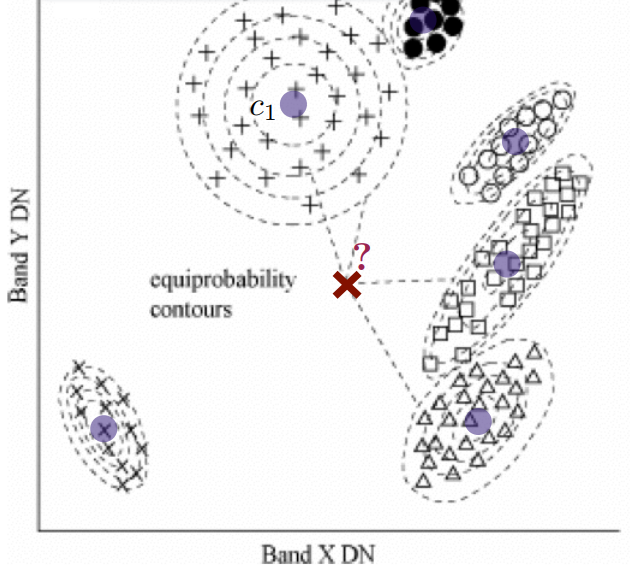
\includegraphics[width=\maxwidth{\linewidth}]{ml_classifier.png}
	\caption{Example of a classifier}
	\label{7-ml-classifier-ex}
\end{figure}

\section{Active contours and level sets}

One of the objective of image segmentation is to extract semantic objects
from the background of the image, in order to process these objects further.
In addition to the feature-based segmentation, other techniques exist.

\subsection{Active contours}

The idea is that we have a curve $\vv{C}(s, t)$ that we want to drive towards
the object frontier in order to extract the object.

In order to drive the movement of this \emph{active contour},
we need an equation of motion:
\begin{equation}
\diffp{\vv{C}}{t}(s, t) = F(\vv{C}(s, t)) \vv{N}(\vv{C}(s, t))
\end{equation}
where $t$ is the time, $s$ is the coordinate of a point along the curve,
$\vv{C}(s, t)$ gives the coordinate of the 1-D point $s$ at time $t$,
$\vv{N}$ is the normal to the curve $\vv{C}$, and $F$ is the acceleration of
(or the force acting on) the point $\vv{C}$ towards the object.
The active contour stops when $F=0$ over all points $s$.

We can decompose $F$ in two components: $F=F_\mathrm{int} + F_\mathrm{ext}$.
\begin{itemize}
	\item $F_\mathrm{int}$ are the internal forces of the curve,
	specifying the tension and smoothness of the contour (function of
	the curvature e.g.)
	\item $F_\mathrm{ext}$ are the external forces that attract the curve
	towards the desired object boundaries.
\end{itemize}

\paragraph{Parametric curves}
In $\R^2$, the curve $\vv{C}\colon [0;1] \mapsto \R^2 \colon p \mapsto
\vv{C}(p) = (x(p), y(p))^\Tr$ has tangent vector
$\vv{T}(p) = \frac{\vv{C}'(p)}{\norm{\vv{C}'(p)}}
= \frac{1}{\sqrt{x'(p)^2+y'(p)^2}} (x'(p), y'(p))^\Tr$
and inward normal vector $\vv{N}(p) = \frac{1}{\sqrt{x'(p)^2+y'(p)^2}} (-y'(p), x'(p))^\Tr$.
We can also define arc length $s$ such that $\norm{\diff{\vv{C}(s)}{s}} = 1$;
that is, $\dif{s} = \norm{\vv{C}'(p)} \dif{p}$ and $\int_{0}^{L} \dif{s} = L$.
We can then define the Frenet curvature $\kappa$ as $\diff{\vv{T}}{s} = \kappa N$,
or $\kappa = \frac{x'y'' - x''y'}{\sqrt{x'^2+y'^2}^3}$.

\paragraph{Active contours types}
There a two types of active contours:
\begin{itemize}
	\item boundary-based active contours, where the local information is given
	by the gradient and we use snakes or geodesic curves as active contours;
	\item region-based active contours, where the local information is given by
	terms depending on the boundary and the region.
\end{itemize}

\subsubsection{Boundary-based active contours}

The basic idea: find $\vv{C}(p)$ minimizing the following energy:
\begin{equation}
E(\vv{C}) = \alpha \int_{0}^{1} \norm{\vv{C}'(p)}^2 \dif{p}
+ \beta \int_{0}^{1} \norm{\vv{C}''(p)}^2 \dif{p}
- \lambda \int_{0}^{1} \norm{\vv{\nabla} I(\vv{C}(p))} \dif{p}.
\end{equation}
The first two terms are the internal energy, constraining the smoothness,
elasticity and rigidity of the curve by means of derivatives,
and the third term is the external energy, attracting the contour towards
the object of the image (the greater the gradient, the better).
$\alpha$, $\beta$ and $\lambda$ are real positive regularization constants.

We can use some calculus to solve this equation and arrive at the following
movement equation:
\begin{equation}
\diffp{\vv{C}(p, t)}{t} = \alpha \diffp{\vv{C}(p, t)}{{p^2}} - \beta \diffp{\vv{C}(p, t)}{{p^4}} + \lambda H(I) \frac{\vv{\nabla}I(\vv{C}(p, t)}{\norm{\vv{\nabla}I(\vv{C}(p, t)}}
\end{equation}
which has a ton of problems:
\begin{itemize}
	\item no topology change allowed;
	\item function not intrisic (depending on the parametrization $p$);
	\item instable numeric scheme requiring $4$-th order derivatives;
	\item needs a close initialization otherwise it will go havoc.
\end{itemize}

Rest of the slides not seen in 2018-2019. But they are interesting.

\subsubsection{Region-based active contours}

Not seen in 2018-2019.

\paragraph{Local and global information} Not seen.

\paragraph{Region-based active contours} Not seen.

\end{document}
